\chapter{Data Visualization with React and D3}
\label{cha:visualization}

The most important aspect of the master's thesis is the thesis project. This chapter introduces the reader to the software and the resulting prototypes that were developed during the implementation phase of the thesis project. A complete walk-through helps the reader to understand the implementation differences of all prototypes. Finally the chapter introduces the reader to the performance testing methodology and the different devices the software was tested on.

\section{Prototypes}

This section introduces the reader to the prototypes of the thesis project. It also explains how the project initially originated. Furthermore every resulting prototype of the project is listed and explained extensively. All in all, the thesis project yielded 3 viable prototypes that are described in this chapter. 

\subsection{Introduction and motivation of the project}

When trying to find the best combination of two libraries, developing prototypes is extremely important. Combining React and D3 in a few different ways in the thesis project ultimately lead to one prototype that then came out on top. The project was primarily realized to provide React developers with an alternative which makes it possible to use D3 force viszalizations by writing React code. Finding a React implementation of D3's force simulation which performs better than the vanilla D3 implementation was not the main goal of the project.

The obvious question "Why do I even need a combination of D3 and React if I could just use pure D3 instead?" can quickly be answered. The initial idea of the project came to mind when a client requested a fully fledged React web application which also included some complex data visualization aspects that are animated in the browser. Instead of having to implement the viszalization part of the application in pure D3, the combination of React and D3 enables all developers of the project to only write declarative D3 code. Using a combination layer API would then result in only one code base that has to be mainitained, instead of two. Also, as mentioned before, D3 tends to become exponentially more difficult to maintain as the project grows.

\subsection{Project setup}

\begin{program}
\caption{Simple example of a React component and its usage} 
\label{prog:forceBuildModule}
\begin{JsCode}
const applyForceHandlers = pipeAppliers(
  applyGeneralForce, 
  applyLinkForce, 
  applyCollisionForce
)

const applyEndHandlers = pipeAppliers(
  applyOnEndHandler, 
  applySimulationReheating
)

const pureD3Updater = pipeAppliers(
  applyNewNodeData,
  applyPureD3Selection,
  applyTickHandler,
  applyForceHandlers,
  applyDragHandlers,
  applyEndHandlers,
)

const hybridUpdater = pipeAppliers(
  applyNewNodeData,
  applyNewRefs,
  applyTickHandler,
  applyForceHandlers,
  applyDragHandlers,
  applyEndHandlers,
)

const pureReactUpdater = pipeAppliers(
  applyNewNodeData, 
  applyForceHandlers, 
  applyEndHandlers
)

const getUpdaterFunction = switchCase({
  [SIMULATION_TYPE.PURE_D3]: pureD3Updater,
  [SIMULATION_TYPE.REACT_D3_HYBRID]: hybridUpdater,
  [SIMULATION_TYPE.PURE_REACT]: pureReactUpdater,
})(null)

export const buildForceSimulation = (options) => {
  const simulation = forceSimulation()
  const updateSimulation = getUpdaterFunction(options.type)
  updateSimulation({ simulation, options })
  return { simulation, updateSimulation }
}
\end{JsCode}
\end{program}

In order to being able to test multiple prototypes one crucial aspect of the project is the force simulation builder setup. All prototypes are built on top of the simulation builder module. The module contains a few D3 specific methods, that allow the developer to build their own force simulation prototype. Some of the methods can be reused by all prototypes and some custom methods have to be implemented per prototype.

By implementing a force simulation builder module it is possible to ensure that all prototype D3 simulations are initialized and updated the exact same way. The most interesting code snippet of the module can be seen in \ref{prog:forceBuildModule}. Individual building blocks of the simulation can simply be piped together because the module uses a functional approach. Lines 12, 21, and 30 show, how the updater functions for the 3 prototypes are composed by using smaller force simulation function blocks.

The most important function in the module of course is the \texttt{buildForceSimulation()} method in line 42 in \ref{prog:forceBuildModule}. The options parameter has to contain a type, which is used to determine what updater function will be applied to the force simulation. The functional switch case statement on line 36 in \ref{prog:forceBuildModule} decides on the basis of the type which updater function to return. The builder function returns an instance of a D3 force simulation and the according updater function, that can be used by each prototype to update the simulation if the data changes.

Another interesting aspect of the code snippet in \ref{prog:forceBuildModule} is, that the functional compositions can be nested. Lines 1 and 7 show the composition of two functions, that con be composed with all three force simulation variants. Even tough they are piped together, the result can then be piped again into every updater function composition as shown in lines 16, 25, and 32 for example where the \texttt{applyForceHandlers} composed method is piped into the updater functions of the different prototypes. Again, the way the updater function composition is implemented ensures the equality of the force simulation initialization of all 3 prototypes.

Of course, due to the fact that all 3 prototypes work fundamentally different, some custom apply functions have to be implemented to ensure the functionality of all 3 prototypes. Applying the custom functions is no problem, as all updater functions are functional compositions. If some custom method has to be added, it can just be applied to the function composition of the according prototype. Line 23 in \ref{prog:forceBuildModule} shows how a custom node reference applying function is composed into the updater function.

Each prototype implements the same API interface and recieves its data via props. All visualization data and each setting parameter therefore has to be passed via props. Using props also means, that the data and the settings must be updateable. The parent container which renders a prototype must be able to update the prototype's data by just passing different props which as a consequence has to be handled correctly in each prototype individually.

\subsection{Pure D3 prototype}

\begin{figure}
\centering
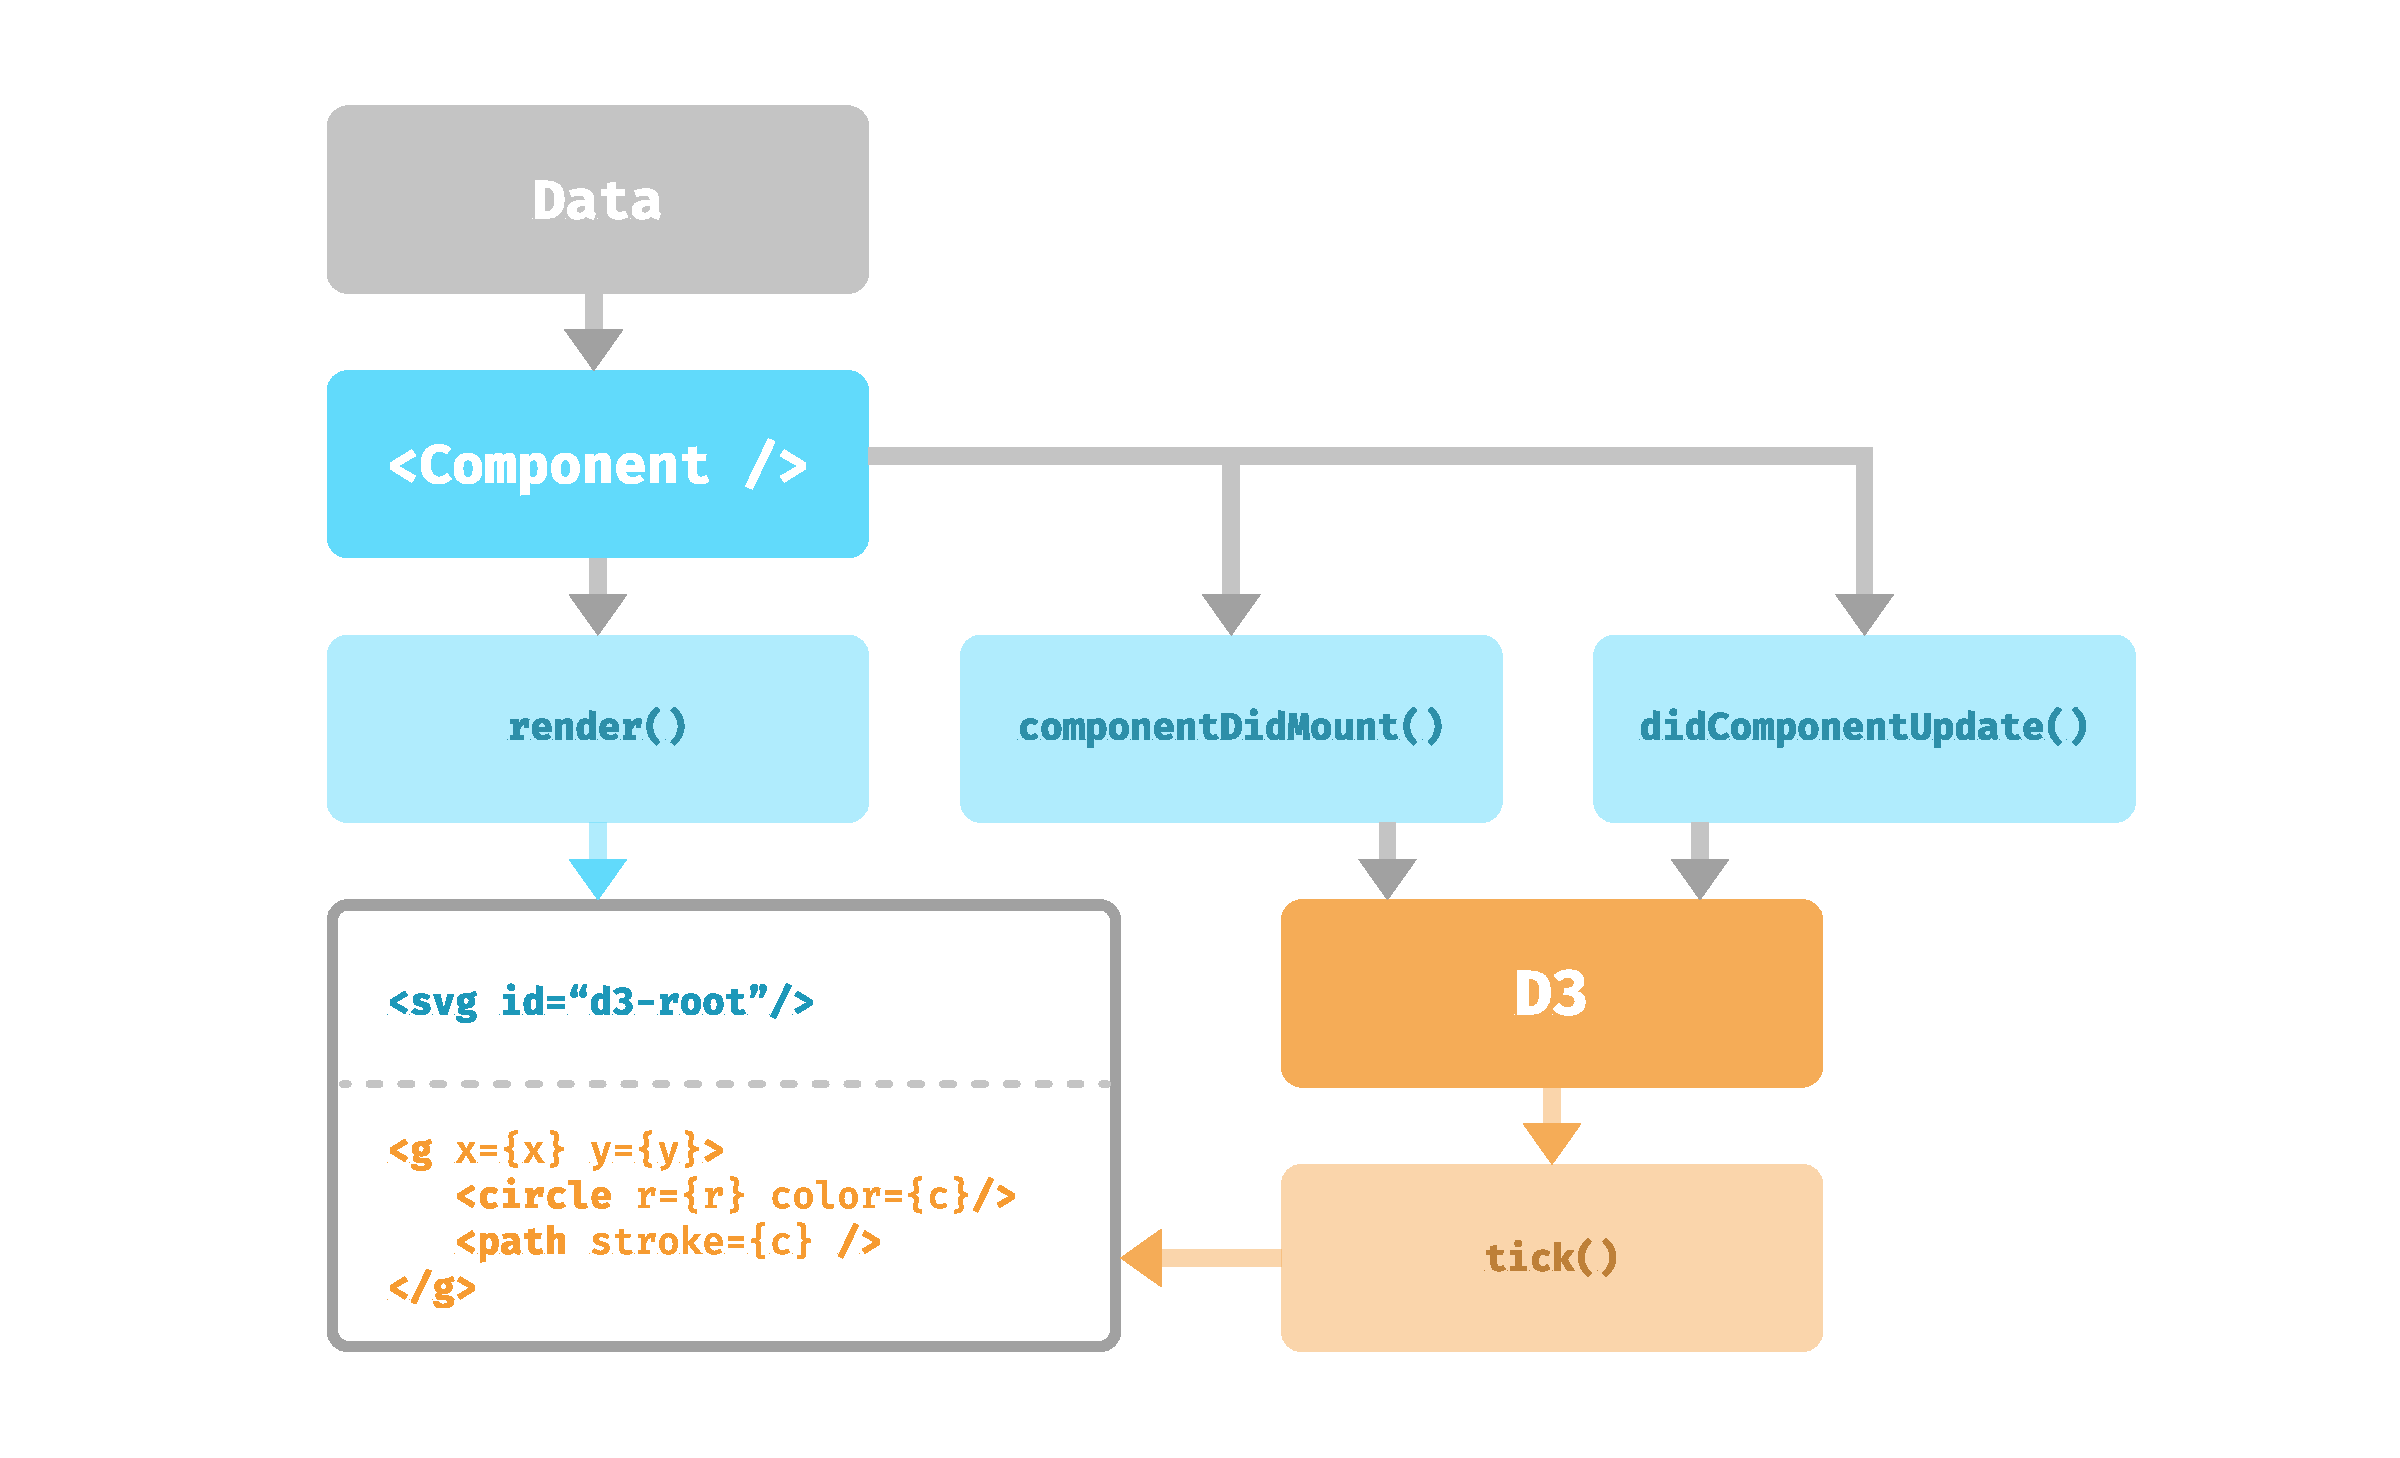
\includegraphics[scale=.6, trim= 4cm 3cm 6cm 3cm, clip, width=1\columnwidth]{impl001.pdf}
\caption{Lifecycle of the pure D3 prototype}
\label{fig:pureD3Lifecycle}
\end{figure}

\begin{program}
\caption{Render function of the pure D3 prototype}
\label{prog:pureD3render}
\begin{JsCode}
render() {
  const { width, height } = this.props
  return <svg ref={this.ref} width={width} height={height} />
}
\end{JsCode}
\end{program}

The first prototype is an experimental implementation. The sole reason of it being realized is to test, if it is even possible to combine React and D3 but still maintaining React's philosophy of unidirectional dataflow and idempotent render function components. The main goal therefore was to create a prototype that would always correctly update itself and thus visualize current data props each render cycle. If the parent component would update the visualization component's data or options the prototype would have to instantly reflect the changes as well. The main difficulty with this prototype is to combine React's declarative approach with D3's imperative way of rendering data.

The implementation heavily relies on the fact, that React's reconciliation algorithm will omit updates to the DOM if the same element is rendered consecutively. The pure D3 graph component only renders a static base SVG as shown in \ref{prog:pureD3render}. After the component mounts, D3 hooks into the base SVG component via the provided ID and builds its own force simulation on top. This means, that D3 will also append and remove the DOM nodes according to the data that was passed to D3. 

As a result React's reconciliation algorithm will not handle nodes that are inside the D3 force simulation if the data changes as the component only renders a static SVG element that will not be updated. Due to the fact, that the SVG element is static, React's reconciliation algorithm will not commit anything to the DOM since every time the render function is called, the SVG tag stays the same. Instead, D3 will fully take over the DOM manipulation and fully handle the simulation by itself without React interfering in any way.

Every time the data updates, the new data is provided directly to D3 via the lifecycle method \texttt{componentDidUpdate()} as figure \ref{fig:pureD3Lifecycle}. Of course each data update will cause React to render the base SVG component but due to the virtual DOM implementation of React the SVG is never newly rendered, as it is static without any dynamic content. The reconciliation algorithm will prevent React from newly committing the SVG tag to the DOM. This fact then enables D3 to work completely separate from React. D3 on the other hand can be implemented like on any other web project as well. Developers must implement the initial force graph generation but also the update logic of course that handles the updated data and applies it to the force graph simulation.

There are 2 component life cycle methods from React that are crucial to this implementation. First, \texttt{componentDidMount()} is used to initialize D3, select the base node and then build the whole force simulation on top. It is important to use the life cycle method that triggers after the initial commit phase, as it makes sure, the component has already been rendered once in order for D3 to being able to select the existing real SVG DOM node. The second important life cycle method is \texttt{componentDidUpdate()} which provides the latest most up to date data directly to D3. That way D3 can then handle the update in the force graph.

\subsubsection{Implmentation details}

\begin{program}
\caption{Pure D3 force graph initializing function}
\label{prog:pureD3InitFn}
\begin{JsCode}
initGraph = () => {
  const { width, height, onSimulationStart } = this.props

  onSimulationStart()

  const svg = select(this.ref.current)
  svg
    .append('g')
    .attr('transform', 'translate(' + width / 2 + ',' + height / 2 + ')')

  const simOptions = this.extractSimOptions()
  const { simulation, updateSimulation } = buildForceSimulation({
    type: SIMULATION_TYPE.PURE_D3,
    ...simOptions,
  })

  this.simulation = simulation
  this.updateSimulation = updateSimulation
}
\end{JsCode}
\end{program}

\begin{program}
\caption{Function that applies the data update to D3 on data changes}
\label{prog:pureD3updateApply}
\begin{JsCode}
applyNodeUpdateCycle = (simulation) => {
  simulation.linkSel.exit().remove()
  
  simulation.linkSel = simulation.linkSel
    .enter()
    .append('path')
    .attr('stroke', '#45b29d')
    .attr('fill', 'none')
    .merge(simulation.linkSel)
  
  let t = transition().duration(750)
  
  simulation.nodeSel
    .exit()
    .style('fill', '#b26745')
    .transition(t)
    .attr('r', 1e-6)
    .remove()
  
  simulation.nodeSel
    .transition(t)
    .style('fill', '#3a403d')
    .attr('r', ({ size }) => size)
  
  simulation.nodeSel = simulation.nodeSel
    .enter()
    .append('circle')
    .style('fill', '#45b29d')
    .attr('r', ({ size }) => size)
    .attr('id', ({ name }) => name)
    .merge(simulation.nodeSel)
}
\end{JsCode}
\end{program}

\begin{program}
\caption{Tick handling function of the pure D3 prototype}
\label{prog:pureD3Tick}
\begin{JsCode}
ticked = () => {
  this.simulation.nodeSel.attr('cx', ({ x }) => x).attr('cy', ({ y }) => y)
  this.simulation.linkSel.attr('d', (d) =>
    this.props.linkType === LINK_TYPES.CURVED ? getCurvedLinkPath(d) : getStraightLinkPath(d),
  )
}
\end{JsCode}
\end{program}

Once the component is initialized, the \texttt{componentDidMount()} lifecycle method directly calls the initializer function which can be seen on line 1 in the code snippet in \ref{prog:pureD3InitFn}. The initializing function appends the base \texttt{<g>} tag and also handles the translation of the current height and width of the component. Then the \texttt{buildForceSimulation()} function is called with the current options and parameters in order to get the simulation and the correct updater function. Note, how the simulation type is passed to the builder function as well. The resulting simulation and updater function is then saved in the current component.

What is also worth mentioning is the fact, that the simulation and the updating function are saved directly to the \texttt{this} context. As stateful components are just plain JavaScript classes, they're capable of having member variables as well. It is of utmost importance not to confuse member variables with React's component state, as React is agnostic to class member variables. React not noticing the member variables does not matter in this case, as we do not want the component to react to the member variables to being able to save state in a component without React going through a new render cycle. 

Looking at the code in \ref{prog:pureD3updateApply}, the update applying functionality can be seen very well. Given a current simulation object, the function will handle all newly entering, transitioning, and exiting nodes accordingly. Even an animation is applied. Each time, the pure D3 react component has updated through the \texttt{componentDidUpdate()} function, the \texttt{applyNodeUpdateCycle()} function is callead. The force simulation building module can take in the updater function and composes it directly into the updating function as seen in line 14 in \ref{prog:forceBuildModule}.

Another vital function of the pure D3 force graph is the tick handler that can be seen in the code snippet in \ref{prog:pureD3Tick}. The ticking function also gets passed to the force simulation builder function. Each iteration of D3's simulation tick the function will then update the position of all nodes and links in the simulation.

\subsubsection{Advantages}

One of the most obvious advantages of the pure D3 force graph implementation is its performance of course. Due to the fact that the implementation uses a native D3 approach to render and update the nodes and links in the simulation, the performance is also comparable to a native D3 implementation. In chapter \ref{cha:performance} the performance is compared to other implementations as well.

\subsubsection{Disadvantages}

The biggest Disadvantage with the pure D3 implementation is the fact, that all DOM manipulations are handled via imperatively chained function calls on the node selections of D3 which also implies, that the node rendering cannot be customized via passing custom render functions for instance. The force graph's code itself has to be changed in order to get different node and link appeareances which leads to the previously described problem of running into unmaintainable code over time.

\subsection{Pure React prototype}

Pure React implementation

\subsection{D3 and React hybrid}

% react move

Hybrid implementation.

\section{Comparison of the different proposed Prototypes}

The implementation of the prototypes is explained.

\section{Building a stable Testing Environment}

The testing environment is explained. Request animation frame testing is explained as well.

\section{Testing methodologies}

I describe how i tested the whole thing

\section{Testing devices}

What devices did i benchmark my prototypes on?
